\documentclass[a4paper]{article}

\usepackage[utf8]{inputenc}
\usepackage[portuges]{babel}
\usepackage{indentfirst}
\usepackage{graphicx}
\usepackage{float}
\usepackage{caption}
\usepackage{subcaption}
\usepackage[T1]{fontenc}
\usepackage{listings}
\renewcommand{\familydefault}{\sfdefault}

\title{Projeto de Computação Gráfica - Fase 1}
\author{Diogo Braga A82547 \and João Silva A82005 \and Ricardo Caçador A81064
\and Ricardo Veloso A81919}
\date{\today}

\begin{document}

\maketitle

\begin{abstract}
Neste relatório é apresentada a primeira fase dum projeto no qual a intenção é desenvolver um mecanismo 3D baseado em gráficos de cenas e fornecer exemplos de uso que mostrem o seu potencial, desenvolvido no âmbito da unidade curricular de Computação Gráfica.
\end{abstract}

\tableofcontents

\newpage


\section{Introdução}
\label{sec:intro}

Esta primeira fase tem como objetivo a criação de duas aplicacões: \textit{generator} e \textit{engine}.
(...)

\section{Generator}
\label{sec:generator}

\subsection{Explicação dos ficheiros criados}
\label{sec:ficheiros}

Cada função recebe como último parâmetro uma string com o nome do ficheiro que vai guardar os pontos que constituem os triângulos necessários para a criação de cada figura.

(...)

\subsection{\textit{Plane}}
\label{sec:plane}
A função \textit{generatePlane} recebe como parâmetro um float que representa o comprimento de cada lado do plano (side).

(...)

\ttfamily
\begin{enumerate}
  \item Atribuir à variavel parcial\_side o valor de side/2
  \item Construir o primeiro triângulo com os pontos:

        \hspace{2cm} P1 $\Rightarrow$ (parcial\_side, 0.0, -parcial\_side)

        \hspace{2cm} P2 $\Rightarrow$ (-parcial\_side, 0.0, -parcial\_side)

        \hspace{2cm} P3 $\Rightarrow$ (-parcial\_side, 0.0, parcial\_side)
  \item Construir o segundo triângulo com os pontos:

        \hspace{2cm} P1 $\Rightarrow$ (parcial\_side, 0.0, -parcial\_side)

        \hspace{2cm} P2 $\Rightarrow$ (-parcial\_side, 0.0, parcial\_side)

        \hspace{2cm} P3 $\Rightarrow$ (parcial\_side, 0.0, parcial\_side)
  \item Fim
\end{enumerate}
\rmfamily


\subsection{\textit{Box}}
\label{sec:box}
A função \textit{generateBox} recebe como parâmetro três float que representam as dimensões de cada eixo da caixa (X, Y e Z), e um inteiro que representa o número de divisões que a caixa tem. (???????????????)

(...)

\subsection{\textit{Sphere}}
\label{sec:sphere}

\subsection{\textit{Cone}}
\label{sec:cone}

\newpage

\section{Engine}
\label{sec:engine}
De forma a representar as figuras de uma determinada cena, usou-se XML para referenciar os ficheiros “.3d” construídos pelo gerador. Esses ficheiros contêm várias pontos que dão resultado a vários triângulos, que resultam em figuras.

\begin{figure}[H]
\centering
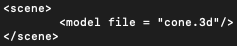
\includegraphics[scale=0.70]{scene_xml.png}
\caption{Exemplo "scene.xml"}
\label{img:scene}
\end{figure}

\section{Câmera}
\label{sec:camera}
De forma a poder visualizar as figuras de diferentes ângulos criamos uma câmera que se encontra fixa enquanto as figuras se movem. Tem tambem a utilidade de ajudar na deteção de erros na criação da figura, caso estes existam. Com recurso às teclas D, A, W, S, Q e E é possível mover a figura para ...

\section{Conclusão}
\label{sec:conclusao}




\end{document}
